\section{Introduction}
Extracting entities and relations from plain texts
is an important and challenging task in natural language processing.
Given a sentence,
the task aims to detect text spans with specific types (\emph{entities})
and semantic relations among those text spans (\emph{relations}).
For example, in the Figure \ref{fig:example},
``Toefting'' is a person entity (\texttt{PER}), 
``teammates'' is a person entity (\texttt{PER}), 
and the two entities have a Person-Social relation (\texttt{PER-SOC}).

To tackle the task of entity relation extraction,
various methods have been proposed,
which can be divided into two categories: pipeline models and joint models.
Pipeline models extract entities and relations in two stages:
entities are first extracted by an entity model,
and then these extracted entities are used as the inputs of a relation model.
Pipeline models often ignore interactions between the two models and 
they suffer from error propagation. Joint models integrate information between entities and relations
into a single model with the joint training,
and have achieved better results than the pipeline models.
In this paper, we focus on joint models.
\begin{figure}[t]
    \begin{center}
        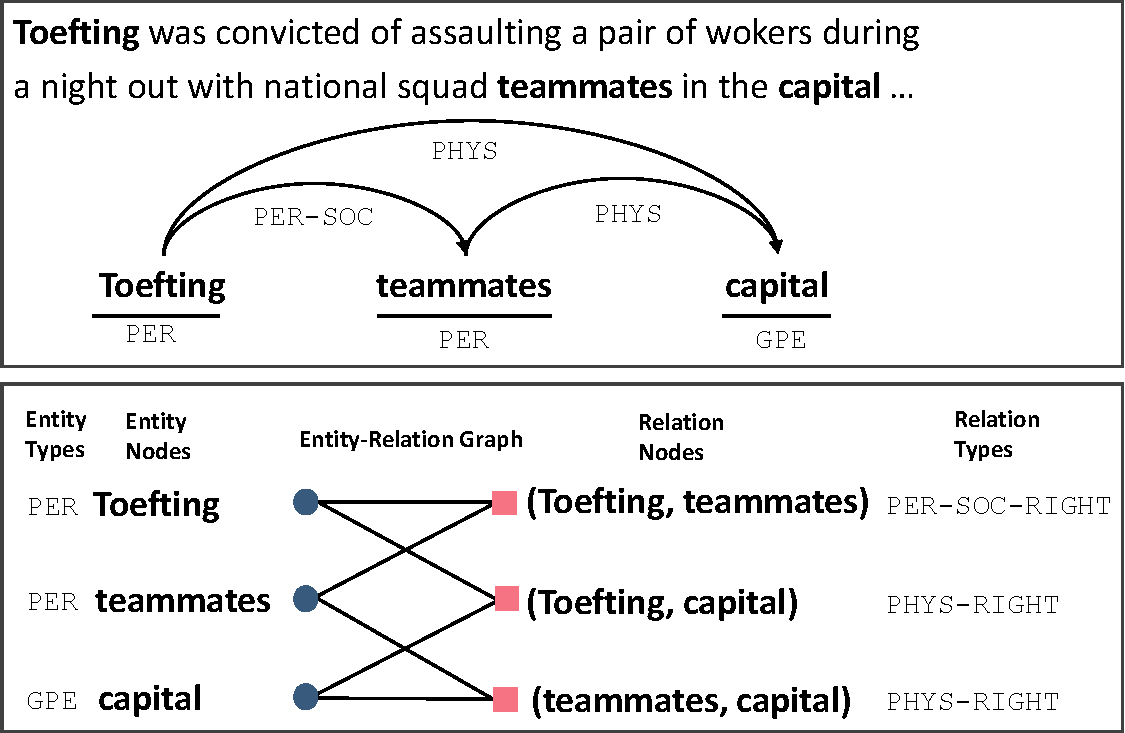
\includegraphics[width=3.0in]{../images/fig-example.pdf}
    \end{center}
    \caption{An example from ACE05. The first part contains annotations
    and the second part is the entity-relation graph of the sentence used in GCN.}
    \label{fig:example}
\end{figure}



More and more joint methods have been applied to this task. 
Among them,
\citet{miwa-bansal:2016:P16-1,katiyar-cardie:2017:Long}
identify the entity with a sequence labelling model,
and identify the relation type with a multi-class classifier.
These joint methods do joint learning through sharing parameters 
and they have no explicit interaction in type inference.
In addition,
some complex joint decoding algorithms 
(e.g., simultaneously decoding entities and relations in beam search) 
have been carefully investigated, including~\citet{li-ji:2014:P14-1,
zhang-zhang-fu:2017:EMNLP2017,zheng-EtAl:2017:Long,wang2018joint}.
They jointly handle span detection and type inference to achieve more interactions.

By inspecting the performance of existing models \cite{D18-1249} on ACE05, 
we find that,
for many entities, their spans are correctly identified,
but their entity types are wrong.
In particular,
the F1 of extracting typed entities is about 83\%,
while the F1 of extracting entity spans is about 90\%.
Thus, if we have a better type inference model,
we may get a better joint extraction performance.
At the same time,
we observe that a joint inference on entity and relation types 
could be potentially better than predicting them independently.
For example, in Figure~\ref{fig:example},
the~\texttt{PER-SOC} relation suggests that the type of  ``Toefting'' might be~\texttt{PER}, and vice versa.
Moreover the \texttt{PER} (``Toefting'') and the relation~\texttt{PER-SOC} could
benefit from other relations such as \texttt{PHYS}.

In this paper,
we define joint entity relation extraction into two sub-tasks:
entity span detection and entity relation type deduction.
For entity span detection,
we treat it as a sequence labeling problem.
For joint type inference,
we propose a novel and concise joint model based on graph convolutional networks (GCNs) \cite{kipf2017semi}.
The two sub-models are trained jointly.
Specifically,
given all detected entity spans in a sentence,
we define an entity-relation bipartite graph.
For each entity span,
we assign an entity node.
For each entity-entity pair,
we assign a relation node.
Edges connect relation nodes and their entity nodes
(last part of Figure \ref{fig:example}).
With efficient graph convolution operations,
we can learn representations for entity nodes and relation nodes
by recursively aggregating information from their neighborhood
over the bipartite graph.
It helps us to concisely capture information among entities and relations.
For example, in Figure \ref{fig:example},
to predict the \texttt{PER} (``Toefting''),
our joint model can pool the information of \texttt{PER-SOC}, \texttt{PHYS},
\texttt{PER} (``teammates'') and \texttt{GPE} (captital).


To further utilize the structure of the graph,
we also propose assigning different weights on graph edges.
In particular,
we introduce a binary relation classification task,
which is to determine whether the two entities form a valid relation.
Different from previous GCN-based models \cite{shang2018end,zhang2018graph},
the adjacency matrix of graph is based on the output of binary relation classification,
which makes the proposed adjacency matrix  more explanatory.
%We compile the proposed joint model with a
%neural network-based model which uses recurrent neural network (RNN) and convolutional neural network (CNN)  similar to~\cite{D18-1249}.
%On  ACE05 dataset,
%we show that the proposed joint model
%is competitive with the state-of-the-art.
To summarize,
the main contributions of this work are
\footnote{ Our implementation is available at  \url{https://github.com/changzhisun/AntNRE}.}
\begin{itemize}[leftmargin=*]
    %\item We define the task of joint entity extraction including entity span detection and entity relation type deduction,
    %which makes it easier to consider the interactions on entity types and relation types jointly. 
    \item We present a novel and concise joint model to handle the joint type inference problem based on graph convolutional network (GCN).
    \item We introduce a binary relation classification task to explore the structure of entity-relation bipartite graph in a more efficient and interpretable way.
    \item We show that the proposed joint model on ACE05
    achieves best entity performance, and is competitive with the state-of-the-art in relation performance.
    
\end{itemize}
